\documentclass[svgnames]{amsart}
\usepackage[paperwidth=6in, paperheight=8in, top = 20mm, bottom = 18mm, left=10mm, right = 10mm]{geometry}

\usepackage{amsmath, amsfonts, amssymb, amsthm}
\usepackage{graphicx, tikz}
\usepackage{mathtools, physics}

\usepackage{enumitem}
\setlist[enumerate,1]{label=\arabic*.}

\usepackage[]{fouriernc}
\usepackage[default,bold]{sourceserifpro}
\usepackage[T1]{fontenc}

\usepackage{xcolor}
\usepackage{scrlayer-scrpage}
\ohead{\color{blue!35!black} \scshape VM}
\cfoot*{\scriptsize\pagemark}

\renewcommand{\th}{\textsuperscript{th}}

\setlength{\parindent}{0pt}

\title[]{Probability and Statistics -- Problem Set 3}

\DeclareMathOperator{\Prob}{P}
\DeclareMathOperator{\EV}{\mathbb E}
\DeclareMathOperator{\Var}{\mathbb V}


\begin{document}
\maketitle
\begin{enumerate}[leftmargin=*, itemsep=0.3em]
\item $X \sim U[a,b]$, $a < 1 < 2 < b$. If $\Prob[X < 1] = 2\Prob[X > 2]$, and $5\Prob[X > 1] = 3\Prob[X < 2]$, find the values of $a$ and $b$.

A fair coin is tossed three times. A player wins $\$1$ if the first toss results in a head, but loses $\$1$ if the first toss results in a tail. Similarly, the player wins $\$2$ if the second toss results in a head, but loses $\$2$ if it results in a tail, and wins or loses $\$3$ according to the result of the third toss. Let $X$ be the total winnings after the three tosses (possibly a negative value if losses are incurred).
\begin{enumerate}
    \item Compute the probability mass function.
    \item Compute the cumulative distribution function.
    \item What is the most likely value of $X$?
\end{enumerate}

\item A contestant on a quiz show is presented with two questions, Questions 1 and 2, which she is to attempt to answer in some order she chooses. If she decides to try Question $i$ first, then she will be allowed to go on to question $j$, $j \neq i$, only if her answer to question $i$ is correct. If her initial answer is incorrect, she is not allowed to answer the other question.

If she is $60$ percent certain of answering Question 1, worth $200$ dollars, correctly and she is $80$ percent certain of answering Question 2, worth 100 dollars, correctly, then which question should she attempt to answer first so as to maximise her expected winnings? Assume that the events $E_i$, $i = 1, 2,$ that she knows the answer to question $i$ are independent
events.

\item The diameter of an electric cable $X$ is assumed to be a continuous random variable with pdf $f(x) = kx (1- x)$, $0 \leq  x \leq 1$.
\begin{enumerate}
    \item Find the value of $k$.
    \item Find the cdf of $X$.
    \item Determine $b$ such that $P(X < b) = 2 P(X \geq b)$.
\end{enumerate}

\item A student takes a multiple choice test consisting of three problems. The first question has $3$ possible answers, the second has $5$ possible answers, and the third question has $4$ possible answers. The student chooses at random one answer as the right one from each of the three problems. Let $X$ be the number of right answers. Find $\EV[X]$ and $\EV[X^2] - \EV[X]^2$.

\item $X$ is a discrete random variable taking values $0, 1, 2, \ldots$, whose pmf $f(x)$ is such that $\dfrac{f(x_1)}{f(x_2)} = r^{x_1 - x_2}$ for all $x_1, x_2 = 0, 1, 2, \ldots$ (where $r \in (0, 1)$ is a constant). Determine $f(x)$ and compute $\EV[X]$.

\item Let $X$ be the random variable with pdf $f(x)$ whose graph is shown below (where $a < b < c$ are three real numbers).\\
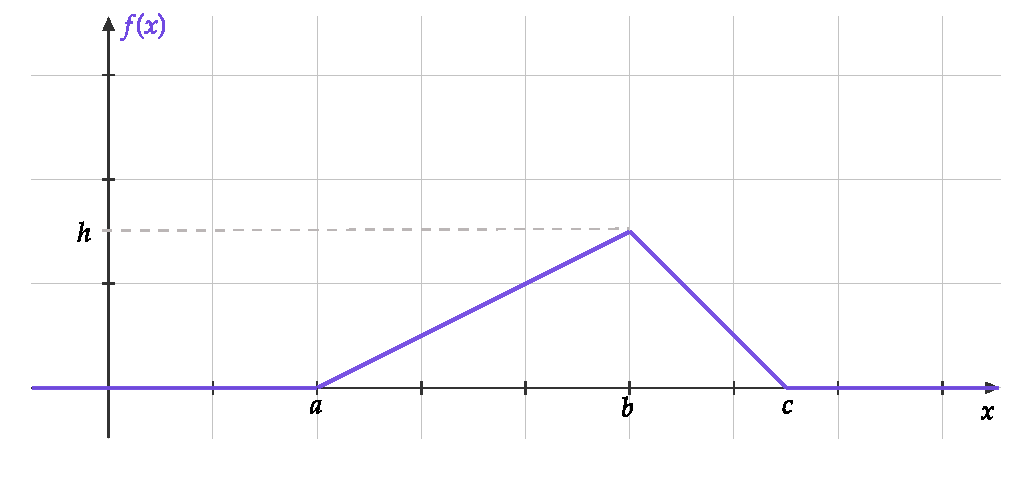
\includegraphics[scale=0.6]{Set3Graph.pdf} \\
Find $h$, and compute $\EV[X]$.

\item Show that the function
\begin{equation*}
f(x) = \dfrac{\lambda^x}{x!}e^{-\lambda}, x = 0, 1, 2, \ldots
\end{equation*}
(where $\lambda > 0$ is a constant) is a valid pmf, and compute $\EV[X]$ and $\Var[X]$.

\item $X$ is a discrete random variable with pmf $f(x) = \dfrac{6}{\pi^2 x^2}$, $x = 1, 2, \ldots$.
\begin{enumerate}
	\item Compute $\Prob[X \ge 3]$
	\item Compute $\Prob[10 \le X \le 15]$
	\item Show that $\EV[X]$ does not exist.
\end{enumerate}

\item $X$ is a continuous random variable with pdf $f(x) = \dfrac 6 {\pi^2} \pqty{\dfrac 1 {\lfloor x \rfloor}}^2$, $x > 1$.
\begin{enumerate}
	\item Compute $\Prob[X \ge 3]$
	\item Compute $\Prob[10 \le X \le 15]$
	\item Show that $\EV[X]$ does not exist.
\end{enumerate}

\item $X$ has pdf $f(x) = \dfrac{x^2}{3}$, $-1 \le x \le 2$. Compute
\begin{enumerate}
	\item $\Prob \bqty{X < \frac 3 2}$
	\item $\Prob[|X| > 1]$
	\item $\Prob \bqty{X < \frac 3 2 \mid X > \frac 1 2}$
	\item $\Prob \bqty{X < \frac 3 2 \mid |X| > 1}$
	\item $\Prob \bqty{|X| < 1 \mid X < \frac 3 2}$.
\end{enumerate}

\item The amount of time in hours that a computer functions before breaking down is a continuous random variable with probability density function given by $f(x) = k e^{\frac{-x}{100}}$, $x \ge 0$.

What is the probability that
\begin{enumerate}
    \item the computer will function between $50$ and $150$ hours before breaking down?
    \item it will function for fewer than $100$ hours?
\end{enumerate}

\item An urn initially has {\color{red} $1$ red} and {\color{blue} $1$ blue} marble. A marble is drawn at random from the urn, and if it is {\color{blue} blue}, it is put back and {\color{red} one red} marble is added to the urn. This is continued until a {\color{red} red} marble is drawn. Let $X$ denote the total number of draws required to obtain a {\color{red} red} marble. Determine the probability distribution of $X$, and find its mean and variance.
{\scriptsize\textbf{Hint}: Compute $\EV[X + 1]$ and $\EV[X^2 - 1]$.}

\item The \emph{median} of a random variable $X$ is the point $c$ such that $\Prob[X \le c] = \Prob[X \ge c] = \frac 1 2$. Compute the median of $X$ with pdf $f(x)$ in each of the following cases.
\begin{enumerate}[itemsep=1em]
	\item $f(x) = \dfrac 1 {b - a}$, $a < x < b$.
	\item $f(x) = a e^{-ax}$, $x > 0$ [where $a > 0$ is a constant].
	\item $f(x) = \dfrac{1}{\pi(1 + x^2)}$ [Note that this distribution has no mean, but has a median].
\end{enumerate}

\item Suppose that if you are $s$ minutes early for an appointment, then you incur the cost $cs$, and if you are $s$ minutes late, then you incur the cost $ks$. Suppose also that the travel time from where you presently are to the location of your appointment is a continuous random variable having probability density function $f$. Determine the time at which you should depart if you want to minimise your expected cost.
\end{enumerate}
\end{document}